% no answer key
% \documentclass[letterpaper]{exam}

% answer key
\documentclass[letterpaper, landscape]{exam}
\usepackage{2in1, lscape} 
\printanswers

\usepackage{units} 
\usepackage{xfrac} 
\usepackage[fleqn]{amsmath}
\usepackage{cancel}
\usepackage{float}
\usepackage{mdwlist}
\usepackage{booktabs}
\usepackage{cancel}
\usepackage{polynom}
\usepackage{caption}
\usepackage{fullpage}
\usepackage{comment}
\usepackage{enumerate}
\usepackage{graphicx}

\newcommand{\dg}{\ensuremath{^\circ}} 
\everymath{\displaystyle}

\title{Calculus I \\ Homework Two \\ Sections 2.1 and 2.2}
\author{}
\date{\today}

\begin{document}

  \maketitle

  \section{Homework}
    \begin{itemize*}
      \item read Section 2.1 and 2.2
      \item exercises: 
        \begin{itemize*}
          \item Section 2.1: 1-3, 10-11, 16
          \item Section 2.2: 4-10, 13-16, 25-29, 32
        \end{itemize*}
    \end{itemize*}

  \ifprintanswers

    \section{Solutions}

    \subsection{Section 2.1}
    \begin{description}

      \item[1]
        \begin{enumerate}[(a)]
          \item \{ -44, -39, -28, -22, -17 \}
          \item $-30$
          \item see Figure \ref{fig:ex01}
        \end{enumerate}

        \begin{figure}[H]
          \centering
          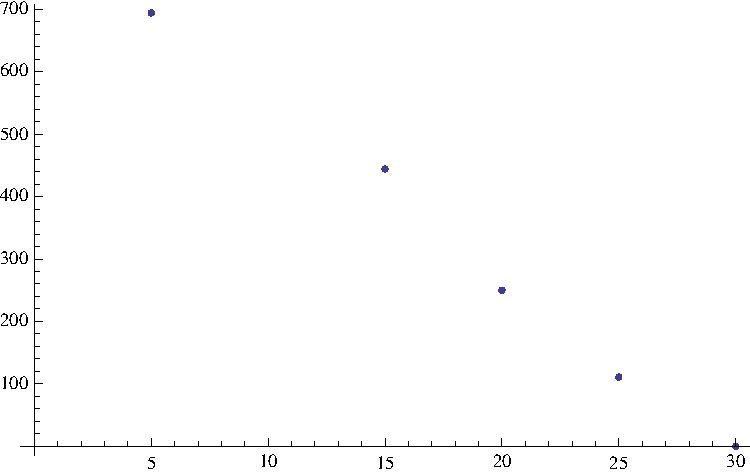
\includegraphics[scale = 0.5]{ex01.pdf}
          \caption{Exercise 1}
          \label{fig:ex01}
        \end{figure}

      \item[2]
        \begin{enumerate}[(a)]
          \item 70
          \item 72
          \item 71
          \item 66
        \end{enumerate}

        The heart rate seems to be declining after minute 42, which is probably
        a good thing.

      \item[3]
        \begin{tabular}[H]{rr}
          \toprule
          x   & slope \\
          \midrule
          0.5 & 0.333333 \\
          0.9 & 0.263158 \\
          0.99 & 0.251256 \\
        \end{tabular}

      \item[10] 
        \begin{enumerate}[(a)]
          \item The slope is the number of degrees the temperature rises each
            year. The T-intercept is the average temperature in 1950.

          \item 2100 is 200 years after 1900. $T(200) = \boxed{ 12.5 \dg }$
        \end{enumerate}

      \item[11] 
        \begin{enumerate}[(a)]
          \item The slope is $\unit[8.34]{mg/yr}$. This is the number of
            additional milligrams of medication to be prescribed for each year
            of age.

          \item The dosage for a newborn is $\boxed{ \unit[8.34]{mg} }$
        \end{enumerate}

      \item[16]
        Find the slope:
        \[
          m = \frac{4800 - 2200}{300 - 200} = \unit[13]{dollars/chair}
        \]

        Use one of the points to find the y-intercept:
        \begin{align*}
          2200 & = 100 \cdot 13 + b \\
          b    & = \unit[900]{chairs} \\
        \end{align*}

        The equation is:
        \[
          y = 13 x + 900
        \]

        \begin{itemize*}
          \item $x$ is the number of chairs produced
          \item $y$ is the cost to produce $x$ chairs
          \item $\unit[13]{dollars/chair}$ is the incremental cost to produce
            one additional chair
          \item \$900 is the cost to pay the rent and keep the factory open,
            even if you aren't producing any chairs.
        \end{itemize*}
    \end{description}

    \subsection{Section 2.2}
    \begin{description}

      \item[4]
        \begin{enumerate}[(a)]
          \item $\lim_{x \to 0} f(x) = 1$
          \item $\lim_{x \to 3^-} f(x) = 4$
          \item $\lim_{x \to 3^+} f(x) = 2$
          \item $\lim_{x \to 3^+} f(x)$ does not exist because the limit is
            different depending on which side you are on
          \item $f(3) = 3$
        \end{enumerate}

      \item[5]
        \begin{enumerate}[(a)]
          \item $\lim_{x \to 1^-} f(x) = 2$
          \item $\lim_{x \to 1^+} f(x) = 3$
          \item $\lim_{x \to 1} f(x)$ does not exist
          \item $\lim_{x \to 5} f(x) = 4$
          \item $f(5)$ is undefined
        \end{enumerate}

      \item[6]
        \begin{enumerate}[(a)]
          \item $\lim_{x \to 0} f(x) = 1$
          \item $\lim_{x \to 3^-} f(x) = 4$
          \item $\lim_{x \to 3^+} f(x) = 2$
          \item $\lim_{x \to 3^+} f(x)$ does not exist because the limit is
            different depending on which side you are on
          \item $f(3) = 3$
        \end{enumerate}

      \item[7]
        \begin{enumerate}[(a)]
          \item $\lim_{t \to 0^-} g(t) = -1$
          \item $\lim_{t \to 0^+} g(t) = -2$
          \item $\lim_{t \to 0^+} g(t)$ does not exist

          \item $\lim_{t \to 2^-} g(t) = 2$
          \item $\lim_{t \to 2^+} g(t) = 0$
          \item $\lim_{t \to 2} g(t)$ does not exist
          \item $g(2) = 0$

          \item $\lim_{t \to 4} g(t) = 3$
        \end{enumerate}

      \item[8]
        \begin{enumerate}[(a)]
          \item $\lim_{x \to 2} R(x) = -\infty$
          \item $\lim_{x \to 5} R(x) = \infty$
          \item $\lim_{x \to 3^-} R(x) = -\infty$
          \item $\lim_{x \to 3^+} R(x) = \infty$

          \item
            \begin{align*}
              x & = -3 \\
              x & = 2 \\
              x & = 5 \\
            \end{align*}

        \end{enumerate}

      \item[10]
        \begin{align*}
          \lim_{t \to 12-} f(t) &= 150 \\
          \lim_{t \to 12+} f(t) &= 300 \\
        \end{align*}

        Before $t = 12$, the level was gradually declining as it was absorbed.
        At $t = 12$ the patient gets a new injection and the level jumps up to 300

      % \item[17]
      %   The values seem to be approaching $\frac{2}{3}$. This makes sense,
      %   because you can simplify the original function to:

      %   \begin{align*}
      %     \frac{x^2 - 2x}{x^2 - x - 2} & = \frac{x (x - 2)}{(x + 1)(x - 2)} \\ & =
      %                                  & = \frac{x}{x + 1} \\
      %   \end{align*}

      %   The function isn't defined at $x = 2$ but it gets closer and closer to
      %   $\frac{2}{3}$ as $x$ gets closer to 2.

      \item[19] The values get close to 0.5.

      \item[21] $\lim_{x \to 0} \frac{\sqrt{x + 4} - 2}{x} = \boxed{ \frac{1}{2} }$ 

      \item[25] $\lim_{x \to -3^+} \frac{x + 2}{x + 3} = \boxed{ -\infty }$ 

      \item[26] $\lim_{x \to -3^-} \frac{x + 2}{x + 3} = \boxed{ \infty }$ 

      \item[27] $\lim_{x \to 1} \frac{2 - x}{(x - 1)^2} = \boxed{ \infty }$ 

      \item[28] $\lim_{x \to 5^-} \frac{e^x}{(x - 5)^3} = \boxed{ -\infty }$ 

      \item[32] 
        \begin{align*}
          \lim_{x \to 2^-} \frac{x^2 - 2x}{x^2 - 4x + 4}   
            & = \lim_{x \to 2^-} \frac{x(x - 2)}{(x - 2)^2} \\
            & = \lim_{x \to 2^-} \frac{x}{x - 2} \\
            & = \boxed{ - \infty } \\
        \end{align*}


    \end{description}

  \else
    \vspace{11 cm}
    \begin{quote}
      \begin{em}
        No cause, however just, can warrant the indiscriminate slaughter that is
        going on minute by minute. I suggest that a cause that demands the
        inhumanities that are being perpetrated today cannot be called just. 
        (on WW II)
      \end{em}
    \end{quote}
    \hspace{1 cm} --Mahatma Gandhi
  \fi

\end{document}

